\documentclass{article}
\usepackage{amsmath}
\usepackage{float}
\usepackage{graphicx}
\usepackage{geometry}
\geometry{hmargin=0.4in, vmargin=0.075in}
\title{ECE 757, Homework 1}
\author{Tudor Popa}
\date{February 2026}

\begin{document}
\maketitle
\section{Profiling and analysis}
To estimate the potential gains of parallelizing \verb|kymppitonni.c|, we used the \verb|getCC()| function to measure the execution time of each game as well as the total execution time of a run with the following parameters:
\begin{itemize}
  \item Games per cutoff: 5000
  \item Minimum cutoff: 10
  \item Maximum cutoff: 300
\end{itemize}
This yielded the given measurements:
\begin{itemize}
  \item $t_{total} = 273550982$ (cycles)
  \item $t_{parallelizable} = 271080903$ (cycles)
\end{itemize}
Using Amdahl's law, we can then estimate theoretical speedups for 1, 2, 4, 8, and 16 processors. The results were calculated using Matlab and are detailed in the graph below.
\begin{figure}[H]
    \centering
    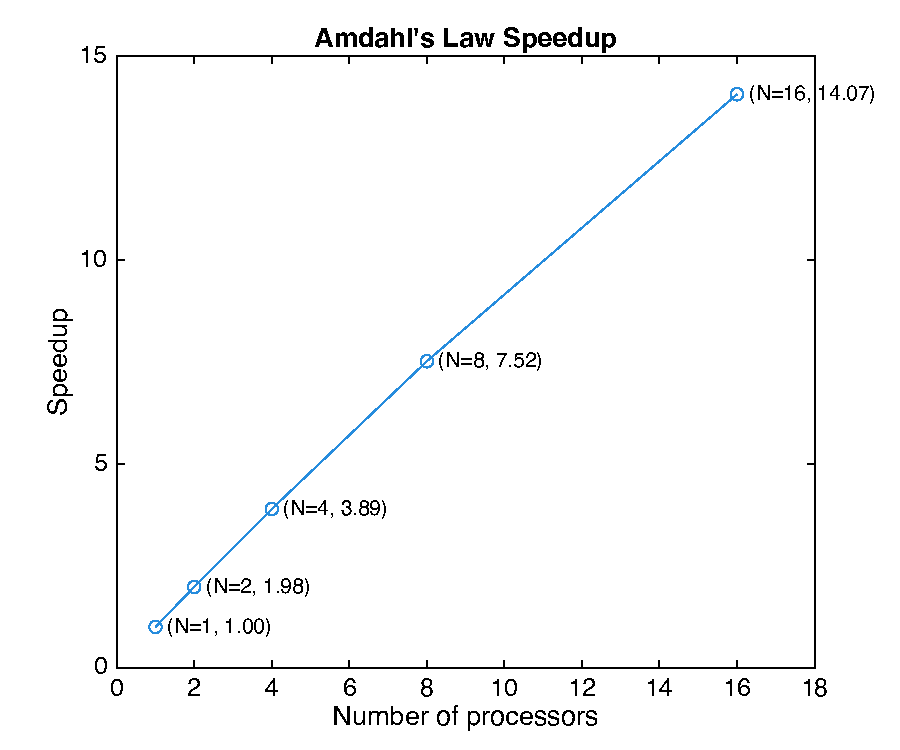
\includegraphics[width=0.45\textwidth]{../outputs/speedup_plot.pdf}
    \caption{Theoretical Amdahl's Law Speedup}
    \label{fig:speedup}
\end{figure}
\section{Running a phtreads parallelized implementation of the game}
The serial version of \verb|kymppitonni.c| was parallelized using pthreads. More specifically, for each cutoff, we ran games in parallel instead of serially. The code was modified to pass the desired number of threads to run as argument.\\
We successively ran it for 2-to-12 threads in increments of 1 with the same number of parameters as before; repeating it 10 times to average the execution times. The results are detailed in the graph below.
\begin{figure}[H]
    \centering
    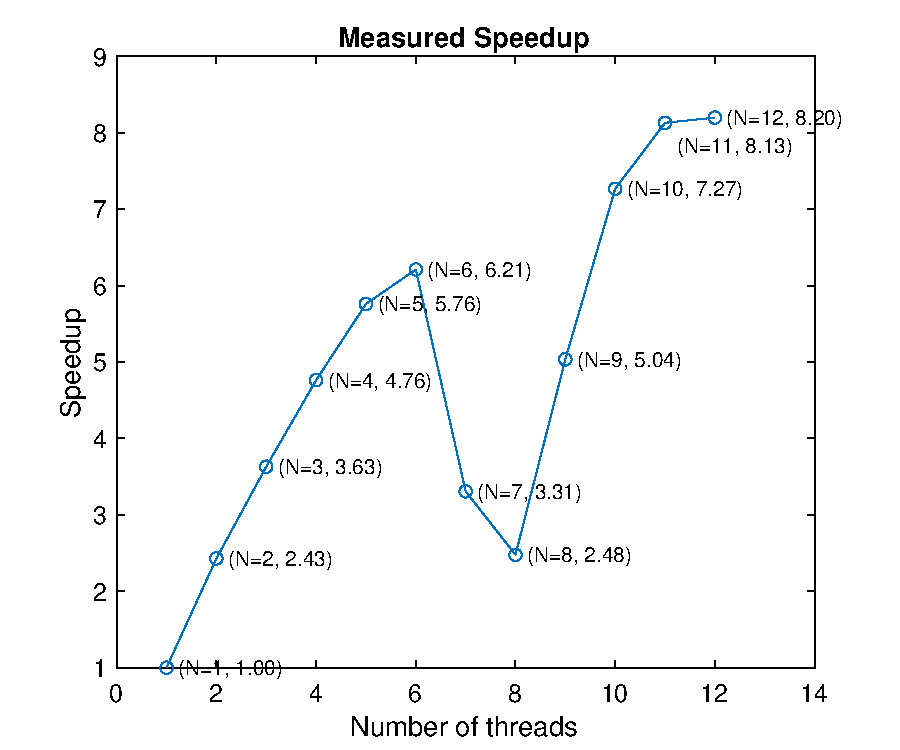
\includegraphics[width=0.45\textwidth]{../outputs/pthreads_plot.pdf}
    \caption{Speedup per number of threads (2-12)}
    \label{fig:pthreads}
\end{figure}
The benchmark was run on a machine with 6 cores and 12 threads. We can observe near linear speedups up to 6 threads, as well as a dip in speedups from 7 to 10 threads. These results appear nominal, given that our test machine only possessed 6 physical threads.
\end{document}
